\chapter{Performanzanalyse}

\section{Qualität}

\section{Geschwindigkeit} \label{sec:speed}

Um die Geschwindigkeit verscheidener Prozessabschnitte und modellen zu testen, bietet es sich
an, die Antwort der KI als Stream zu betrachten, da dieser in Echtzeit ausgewertet werden kann.
So kann zum Beispiel auch untersucht werden bei welche modellen die Textgenerierung und bei
welchen die Diagrammgenereirung schneller ist.
Um sich aber nur auf gestreamte Daten zu begrenzen, muss zunächst festgestellt werden, ob
sich die Generierungszeiten eines LLM Anbieters unterscheiden, wenn man stream bzw. nicht 
streamt.

Dafür werden nun in Abbildung \ref{fig:timing-streaming} einige Modelle getestet, ob sich die Zeiten 
jeweils stark unterscheiden.
Hierfür wird folgender Prompt verwendet:

\begin{prompt}
\noindent\fbox{
  \parbox{\textwidth}{
    Erstelle eine Prozessbeschreibung eines Beliebigen Prozesses mit 95 bis 105 Wörtern welche 
    5 tasks, 1 gateway und 2 message flows beinhaltet.
    Setzte diese dann direkt in ein Diagramm um. Das Diagramm soll nur genau die 5 tasks, 1 
    gateway und 2 message flows beinhalten, mehr nicht.
  }
}
\label{prompt:speed}
\caption{Prompt für einen Geschwindigkeitstest}
\end{prompt}

\begin{figure}[H]
\centering
\pgfplotstableread{ % data 
Model	           Gestreamt   NichtGestreamt
Gemini-2.5-Pro	    44.852	    45.322
Gemini-2.5-Flash	38.364	    39.091
Grok-3	            52.668	    55.567
Grok-3-Fast	        53.252	    59.121
ChatGPT-4.1	        46.938	    47.810
ChatGPT-5-Mini	   207.647	   216.427
Claude-Sonnet-4.5	52.913	    53.079 
}\datastreamnostream
\pgfplotstablesort[sort key=Gestreamt, sort cmp=float <]{\sorteddatastreamnostream}{\datastreamnostream}
\begin{tikzpicture}
\begin{axis}[
    xbar,   % Dual horizontal bars
    width=.8\textwidth,
    xmin=0,         
    ytick=data,     
    bar width=4mm,
    y=11mm,
    enlarge y limits=0.1,
    legend style={
        legend columns=2,
        at={(0.5,0)},   
        anchor=north,
        yshift=-3em,
        draw=none
    },
    area legend,
    xlabel={Zeit [Sekunden]},
    yticklabels from table={\sorteddatastreamnostream}{Model}, 
    tick label style={font=\footnotesize}
]
\addplot [fill=green!60,
    point meta=x,
    nodes near coords,
    nodes near coords align={anchor=west},
    every node near coord/.append style={
        black,
        fill=white,
        fill opacity=0.75,
        text opacity=1,
    }
] table [x=Gestreamt, meta=Model,y expr=\coordindex] {\sorteddatastreamnostream};   
\addplot [fill=red!60,
    point meta=x,
    nodes near coords,
    nodes near coords align={anchor=west},
    every node near coord/.append style={
        black,
        fill=white,
        fill opacity=0.75,
        text opacity=1,
    }
] table [x=NichtGestreamt, meta=Model,y expr=\coordindex] {\sorteddatastreamnostream};
\legend{Gestreamt,Nicht Gestreamt}
\end{axis}
\end{tikzpicture}
\caption{Zeitperformanzvergleich Gestreamt vs Nicht Gestreamt}
\label{fig:timing-streaming}
\end{figure}

Aus diesen Daten geht hervor, dass bei jedem Modell die Variante des Streamings die Variante 
ohne Streamings in Bezug auf Geschwindigkeit überbietet.
Der Unterschied beträgt jeweils unter 10\%.
Damit ist nun klar, dass die Variante des Stremings nicht der Variante Ohne Streamings unterliegt
und für weitere Tests kann die Variante des Streamings verwendet werden während die Nicht 
Streaming Variante vernachlässigt wird.

Als nächstes soll nun untersucht werden welcher der zwei implementierten Formate \texttt{JSON}
und \texttt{XML} sich Zeitlich besser verhält.
In Abbildung \ref{fig:timing-xmljson} wird für das Promptbeispiel auf Seite \pageref{prompt:speed} dieses Verhalten 
getestet.

\begin{figure}[H]
\centering
\pgfplotstableread{ 
Model	Antwort	StreamInitialisierung	Text	Diagramm	Formatierung	Datenbank
XML	    28.345	0.004                   0.194	24.949	    0	            0.671
JSON	28.453	0.001	                0.189	13.707	    0.009	        0.554
}\dataxmljson
\begin{tikzpicture}
\begin{axis}[
    xbar stacked,   % Stacked horizontal bars
    width=.9\textwidth,
    xmin=0,         
    ytick=data,     
    bar width=6mm,
    y=8mm,
    enlarge y limits=0.8,
    legend style={
        legend columns=4,
        at={(0.5,0)},   
        anchor=north,
        yshift=-3em,
        draw=none
    },
    area legend,
    xlabel={Zeit [Sekunden]},
    yticklabels from table={\dataxmljson}{Model}  
]
\addplot [fill=green!60] table [x=Antwort, meta=Model,y expr=\coordindex] {\dataxmljson};   
\addplot [fill=blue!60] table [x=StreamInitialisierung, meta=Model,y expr=\coordindex] {\dataxmljson};
\addplot [fill=magenta!60] table [x=Text, meta=Model,y expr=\coordindex] {\dataxmljson};   
\addplot [fill=orange!60] table [x=Diagramm, meta=Model,y expr=\coordindex] {\dataxmljson};   
\addplot [fill=purple!60] table [x=Formatierung, meta=Model,y expr=\coordindex] {\dataxmljson};   

\addplot [fill=red!60,
    point meta=x,
    nodes near coords,
    nodes near coords align={anchor=west},
    every node near coord/.append style={
        black,
        fill=white,
        fill opacity=0.75,
        text opacity=1,
    }
] table [x=Datenbank, meta=Model,y expr=\coordindex] {\dataxmljson};
\legend{Antwort,Streamstart,Textgenerierung,Diagrammgenerierung,Formatierung,Datenbankaufruf}
\end{axis}
\end{tikzpicture}
\caption{Zeitperformanzvergleich JSON vs XML bei Gemini 2.5 Pro}
\label{fig:timing-xmljson}
\end{figure}

Man erkannt einfach, dass die Diagrammgenerierung bei JSON um einiges schneller ist als bei XML.
Der Konvertierungsprozess von JSON zu XML beträgt in diesem Beispiel nur 9 ms und ist damit um
einiges effizienter als die um 11242 ms längere Diagrammgenerierung bei XML.

Interessant ist nun noch zu sehen wie diese Aufwandsdifferenz von der Größe des Diagramms abhängt.
Hierfür wird nun in Abbildung \ref{fig:timing-xmljson-elements} Gemini 2.5 Pro im Quick modus benutzt um 
verschieden große Diagramme zu erzeugen.
Hierfür wird folgender Prompt verwendet:

\begin{prompt}[H]
\noindent\fbox{
  \parbox{\textwidth}{
    Erstelle ein BPMN Diagramm für ein Prozess deiner Wahl. 
    Sei kreativ.
    Benutze insgesamt genau [anzahl-elemente] Elemente wie z.B. Tasks, Gates, End-Events, 
    Message-Flows, Pools, Lanes, etc.
  }
}
\label{prompt:speed-elements}
\caption{Prompt für einen Diagramm-Geschwindigkeitstest nach Größe}
\end{prompt}


\begin{figure}[H]
\centering
\pgfplotstableread{ 
Elemente	XML	    JSON
2	        5.567	2.444
5	        7.302	3.816
10	        13.594	8.489
20	        26.565	16.049
50	        80.995	36.091
}\dataxmljson
\begin{tikzpicture}
\begin{axis}[
    xtick=data,
    width=.9\textwidth,
    xmin=0,
    ymin=0,
    enlarge y limits=0,
    legend style={
        legend columns=4,
        at={(0.5,0)},   
        anchor=north,
        yshift=-3em,
        draw=none
    },
    area legend,
    xlabel={Anzahl Elemente},
    ylabel={Zeit [Sekunden]},
]
\addlegendentry{XML};
\addplot [smooth,mark=*,color=blue!60] table [y=XML, x=Elemente] {\dataxmljson};
\addlegendentry{JSON};
\addplot [smooth,mark=*,color=red!60] table [y=JSON, x=Elemente] {\dataxmljson};
\end{axis}
\end{tikzpicture}
\caption{Zeitperformanzvergleich JSON vs XML bei Gemini 2.5 Pro nach Anzahl der Elemente (Nur Diagramm)}
\label{fig:timing-xmljson-elements}
\end{figure}

Die Auswertung der gemessenen Laufzeiten in Abbildung \ref{fig:timing-xmljson-elements} zeigt 
deutlich, dass die Diagrammgenerierung im 
JSON-Format gegenüber dem XML-Format einen spürbaren Geschwindigkeitsvorteil bietet. 
Insbesondere bei zunehmender Diagrammgröße wächst der Unterschied merklich.  
In den meisten Testfällen liegt die Generierungsdauer des JSON-Modells bei ungefähr der Hälfte 
der Zeit, die für die entsprechende XML-Ausgabe erforderlich ist. 
Dieser Geschwindigkeitsvorteil lässt sich vor allem auf die kompaktere Syntax und die geringere 
Redundanz zurückführen. 
Insgesamt wird dadurch klar, dass JSON für performanzkritische Anwendungsfälle, 
insbesondere bei großen oder komplexen Diagrammen, erhebliche Vorteile bietet.

Weitergehend soll nun untersucht werden welche Modelle sich für eine Zeiteffiziente 
Generierung eignen. Dafür werden in Abbildung \ref{fig:timing-models} einige gänige Modelle
getestet.

\begin{figure}[h]
\centering
\pgfplotstableread{ 
Model	            Antwort	StreamInitialisierung	Text	Diagramm	Formatierung	Datenbank
Gemini-2.5-Pro	    34.396	000.001	                0.433	15.274	    0.005	        0.554
Gemini-2.5-Flash	36.529	000.002	                0.162	07.292	    0.005	        0.512
Grok-3	            00.003	006.203	                0.418	16.850	    0.005	        0.510
Grok-3-Fast	        00.004	005.056	                0.386	14.853	    0.007	        0.508
ChatGPT-4.1	        00.904	001.138	                0.232	18.051	    0.003	        0.580
ChatGPT-5-Mini	    01.874	115.226	                0.414	22.258	    0.007	        0.580
Claude-Sonnet-4.5	04.370	000.001	                0.906	16.903	    0.006	        0.582
}\datamodels
\pgfplotstableset{
    create on use/Total/.style={
        create col/expr={\thisrow{Antwort} + \thisrow{StreamInitialisierung} + \thisrow{Text} + \thisrow{Diagramm} + \thisrow{Formatierung} + \thisrow{Datenbank}}
    }
}
\pgfplotstablesort[sort key=Total, sort cmp=float <]{\sorteddatamodels}{\datamodels}
\begin{tikzpicture}
\begin{axis}[
    xbar stacked,   % Stacked horizontal bars
    width=.9\textwidth,
    xmin=0,         
    ytick=data,     
    bar width=6mm,
    y=8mm,
    enlarge y limits=0.15,
    legend style={
        legend columns=4,
        at={(0.5,0)},   
        anchor=north,
        yshift=-3em,
        draw=none
    },
    area legend,
    xlabel={Zeit [Sekunden]},
    yticklabels from table={\sorteddatamodels}{Model}  
]
\addplot [fill=green!60] table [x=Antwort, meta=Model,y expr=\coordindex] {\sorteddatamodels};   
\addplot [fill=blue!60] table [x=StreamInitialisierung, meta=Model,y expr=\coordindex] {\sorteddatamodels};
\addplot [fill=magenta!60] table [x=Text, meta=Model,y expr=\coordindex] {\sorteddatamodels};   
\addplot [fill=orange!60] table [x=Diagramm, meta=Model,y expr=\coordindex] {\sorteddatamodels};   
\addplot [fill=purple!60] table [x=Formatierung, meta=Model,y expr=\coordindex] {\sorteddatamodels};   

\addplot [fill=red!60,
    point meta=x,
    nodes near coords,
    nodes near coords align={anchor=west},
    every node near coord/.append style={
        black,
        fill=white,
        fill opacity=0.75,
        text opacity=1,
    }
] table [x=Datenbank, meta=Model,y expr=\coordindex] {\sorteddatamodels};
\legend{Antwort,Streamstart,Textgenerierung,Diagrammgenerierung,Formatierung,Datenbankaufruf}
\end{axis}
\end{tikzpicture}
\caption{Zeitperformanzvergleich verschiedener Modelle}
\label{fig:timing-models}
\end{figure}

Auffällig in Abbildung \ref{fig:timing-models} ist, dass ChatGPT-5-Mini mit großem Abstand die 
längste Gesamtzeit benötigt
Besonders der Streamstart dauert extrem lange, was darauf hindeutet, dass dieses Modell trotz 
möglicher inhaltlicher Stärke für eine schnelle Generierung ungeeignet ist. 
Die beiden Gemini-2.5-Modelle liegen im mittleren Bereich und zeigen ihre Stärken vor allem in 
der schnellen eigentlichen Antwortphase und soliden Textgenerierung, verlieren jedoch viel Zeit 
dabei die Anfrage anzuhmen und die Antwort zu übersenden. 
Grok-3, Grok-3-Fast, Claude-Sonnet-4.5 und ChatGPT-4.1 zeigen die insgesamt ausgewogenste 
Performance, da keine der Einzeldisziplinen überproportional viel Zeit beansprucht. 
Besonders Grok-3-Fast und ChatGPT-4.1 sind nahezu gleich schnell und deutlich effizienter als die 
größeren Modelle; sie zeichnen sich durch kurze Streamstart-Phasen und schnelle Diagramm- und 
Texterstellung aus.  
Insgesamt zeigen die kompakten oder speziell optimierten Modelle eine hohe 
Reaktionsgeschwindigkeit über alle Teilschritte hinweg, während größere Modelle wie 
ChatGPT-5-Mini und die Gemini-Reihe durch längere Initialisierungen ausgebremst werden. 

\section{Kosten}

\begin{table}[h!]
    \centering
    \begin{tabular}{llrrr}
        \toprule
        Provider & Model & Input & Cached Input & Output \\
        \midrule
        OpenAI & gpt-5.1 & 1.25 \$ & 0.13 \$ & 10.00 \$ \\
        OpenAI & gpt-5 & 1.25 \$ & 0.13 \$ & 10.00 \$ \\
        OpenAI & gpt-5-mini & 0.25 \$ & 0.03 \$ & 2.00 \$ \\
        OpenAI & gpt-5-nano & 0.05 \$ & 0.01 \$ & 0.40 \$ \\
        OpenAI & gpt-5-pro & 15.00 \$ & 0.00 \$ & 120.00 \$ \\
        OpenAI & gpt-4.1 & 2.00 \$ & 0.50 \$ & 8.00 \$ \\
        OpenAI & gpt-4.1-mini & 0.40 \$ & 0.10 \$ & 1.60 \$ \\
        OpenAI & gpt-4.1-nano & 0.10 \$ & 0.03 \$ & 0.40 \$ \\
        OpenAI & gpt-4o & 2.50 \$ & 1.25 \$ & 10.00 \$ \\
        OpenAI & gpt-4o-mini & 0.15 \$ & 0.08 \$ & 0.60 \$ \\
        \midrule
        Anthropic & claude-opus-4-1 & 15.00 \$ & 1.50 \$ & 75.00 \$ \\
        Anthropic & claude-sonnet-4-5 & 3.00 \$ & 0.30 \$ & 15.00 \$ \\
        Anthropic & claude-haiku-4-5 & 1.00 \$ & 0.10 \$ & 5.00 \$ \\
        Anthropic & claude-sonnet-4 & 3.00 \$ & 0.30 \$ & 15.00 \$ \\
        Anthropic & claude-opus-4 & 15.00 \$ & 1.50 \$ & 75.00 \$ \\
        Anthropic & claude-sonnet-3-7 & 3.00 \$ & 0.30 \$ & 15.00 \$ \\
        Anthropic & claude-haiku-3-5 & 0.80 \$ & 0.08 \$ & 4.00 \$ \\
        Anthropic & claude-opus-3 & 15.00 \$ & 1.50 \$ & 75.00 \$ \\
        \midrule
        xAI & grok-4-1-fast-reasoning & 0.20 \$ & 0.05 \$ & 0.50 \$ \\
        xAI & grok-4-1-fast-non-reasoning & 0.20 \$ & 0.05 \$ & 0.50 \$ \\
        xAI & grok-4-fast-reasoning & 0.20 \$ & 0.05 \$ & 0.50 \$ \\
        xAI & grok-4-fast-non-reasoning & 0.20 \$ & 0.05 \$ & 0.50 \$ \\
        xAI & grok-4 & 3.00 \$ & 0.05 \$ & 15.00 \$ \\
        xAI & grok-3-mini & 0.30 \$ & 0.08 \$ & 0.50 \$ \\
        xAI & grok-3 & 3.00 \$ & 0.75 \$ & 15.00 \$ \\
        \midrule
        Google & gemini-2.5-pro & 0.00 \$ & 0.00 \$ & 0.00 \$ \\
        Google & gemini-2.5-flash & 0.00 \$ & 0.00 \$ & 0.00 \$ \\
        Google & gemini-2.5-flash-lite & 0.00 \$ & 0.00 \$ & 0.00 \$ \\
        Google & gemini-2.0-flash & 0.00 \$ & 0.00 \$ & 0.00 \$ \\
        \bottomrule
    \end{tabular}
    \caption{Tokenpreise pro 1M Token \\ (Stand: 20.11.2025)}
    \label{tab:tokenpreise}
\end{table}

Die Tabelle \ref{tab:tokenpreise} zeigt einen Überblick über die Tokenpreise der 
KI-Modellanbieter, welche implementiert wurden, im Stand von November 2025.
Jeder Modellanbieter hat eine breite Abdeckung an Modellen mit unterschiedlichen Preisen.
Hierbei gibt es oftmals ein  billiges Modell, welches möglicherweise qualitativ
schlechtere Ergebnisse erziehlt und ein teureres Modell, welches qualitativ besser ist.
Über alle Modelle hinweg wird aber klar, dass Tokens, welche für den Output verwendet werden,
mit Abstand am teuersten sind, während Tokens für den Input generell eher billiger sind.

Die Gemini kostenlose Stufe bietet den Vorteil, dass man manche Gemini Modelle, darunter 
Gemini 2.5, völlig kostenlos nutzen kann. 
Allerdings gibt es hier auch Nachteile: 
Laut offizieller Rate-Limits sind beispielsweise bei Gemini 2.5 Flash nur 10 Anfragen pro 
Minute und 250 Anfragen pro Tag erlaubt. 

Betrachtet man nun eine Diagrammerstellung mit dem Prompt von Seite \pageref{prompt:speed},
kann man sehen wie sich die Menge der Tokens Für Input und Output auf den Preis auswirken.
In Diagramm \ref{fig:price-gen-1} wurde Beispielsweise GPT-4.1 verwendet um ein Diagramm zu 
erstellen.

\begin{figure}[h]
    \centering
    \begin{tikzpicture}
        \pie[pos ={0,0}, radius=2, sum=0.0466, after number=\space\$]{0.0235/input, 0.0231/output}
        \pie[pos ={5,0}, radius=2, sum=0.1018, after number=\space\$]{0.0775/input, 0.0243/output}
    \end{tikzpicture}
    \caption{Kosten für die erste und fünfte Diagrammerstellung im Thread}
    \label{fig:price-gen-1}
\end{figure}

Wie man sieht sind, obwohl die input token preise um einiges billiger sind als die output token 
preise, die Kosten des Inputs für eine Diagrammerstellung in der ersten Nachricht mehr als 50\%.
In der fünften Nachricht sind die Input Token Kosten bereits bei über 75\%.
Während die Kosten für das erste Diagramm noch 0.0466 \$ betragen, sind es bei der fünften Nachricht
schon 0.1018 \$. 
Da der Input bei Folgenachrichten zum Großteil der gleiche ist, wie der bei Nachrichten davor,
Bieten viele LLM Anbieter eine Funktionalität des \texttt{Input Caching} an. 

Input zu cachen kann viel bringen, wenn sich Teile einer Anfrage immer wiederholen. 
Viele Inhalte der Anfragen ist dem LLM Anbieter durch vorherige ANchrichten in einem Thread bereits bekannt. 
Diese Inhalte jedes Mal neu an das Modell zu schicken, kostet viele Tokens und damit Geld. 
Wenn der Input aber gecacht wird, kann das Modell auf eine bereits gespeicherte interne 
Darstellung zurückgreifen. 
Dadurch muss es die Daten nicht noch einmal vollständig verarbeiten.

Die Tabelle \ref{tab:tokenpreise} zeigt, dass gecachter Input bei vielen Modellen deutlich 
günstiger ist als normaler Input, bei manchen Modellen sogar gar nichts. 
Das bedeutet: Je mehr wiederverwendete Daten eine Anfrage hat, desto stärker sinken die 
Gesamtkosten. 
Gleichzeitig antwortet das Modell schneller, weil weniger berechnet werden muss.

\begin{figure}[h]
    \centering
    \begin{tikzpicture}
        \pie[pos ={0,0}, radius=2, sum=0.0466, after number=\space\$]{0.0235/input, 0.0231/output}
        \pie[pos ={5,0}, radius=2, sum=0.0578, after number=\space\$]{0.0065/input,  0.0240/output, 0.0272/cached input}
    \end{tikzpicture}
    \caption{Kosten für die erste und fünfte Diagrammerstellung im Thread mit Input-Caching}
    \label{fig:price-gen-2}
\end{figure}

Man sieht in Abbildung \ref{fig:price-gen-2} gut, dass das Caching des Inputs viel Geld sparen 
kann.
Während in diesem Beispiel das fünfte Diagramm ohne Caching noch 0.1018 \$ gekostet hat,
hat das fünfte Diagramm mit Caching nur noch 0.0578 \$ gekostet.
Für dieses Beispiel hat sich Caching sehr gelohnt.

Das Caching hat aber für den BPMN Bot nur begrenzt einen Effekt.
Es ist Teil der Software, dass der Nutzer das KI Modell komplett frei wählen kann.
Dies kann er auch innerhalb eines Threads bei jeder neuen Nachricht entscheiden und ist dabei nicht
an einen Anbieter gebunden.
Dadurch muss bei einem Modellwechsel trotzdem der gesamte Threadkontext an das neue Modell
gesendet werden.

Zusammenfassend lässt sich festhalten, dass es verschiedene Strategien gibt, 
die Kosten für die Nutzung von KI-Modellen zu reduzieren. 
Ein naheliegender Ansatz ist die Auswahl eines Modells mit niedrigen Tokenpreisen. 
Dabei besteht jedoch immer das Risiko, dass günstigere Modelle auch qualitativ schwächere 
Ergebnisse liefern. 
Für bestimmte Anwendungsfälle mag dies ausreichend sein, bei komplexeren Diagrammen kann es 
jedoch zu deutlichen Qualitätseinbußen kommen.

Eine weitere Möglichkeit bietet das kostenfreie Gemini-Angebot. 
Allerdings bringt die kostenlose Stufe klare Einschränkungen mit sich, insbesondere die 
strengen Limits an täglichen und minütlichen Anfragen. 
Dadurch wird die skalierung der Software auf eine große Nutzeranzahl verhindert.

Auch das Input-Caching kann eine wirksame Methode zur Kostenreduzierung sein. 
Insbesondere bei langen Chats, kann das Caching den Preis pro Anfrage deutlich senken. 
Gleichzeitig verbessert sich die Antwortgeschwindigkeit, da bereits bekannte Inhalte nicht 
erneut ausgewertet werden müssen. 
Allerdings entfaltet Caching seine Vorteile nur dann, wenn innerhalb eines Threads durchgehend 
derselbe Modellanbieter verwendet wird. 
Da der BPMN-Bot dem Nutzer jedoch volle Flexibilität bei der Modellwahl lässt, 
einschließlich eines Modellwechsels mitten im Gespräch, muss beim Wechsel weiterhin der 
komplette Kontext erneut übertragen werden. 
Dadurch verliert das Caching in solchen Situationen an Effektivität.

Wie auch schon im Kapitel \ref{sec:speed} besprochen, hat auch die Wahl des Diagrammformats eine
entscheidenden Rolle.
Die Nutzung von JSON gegenüber XML kann eine Einsparung von bis zu etwa 50\% der Output
Token bewirken, wodurch weiter einiges an Kosten gespart werden kann.

Insgesamt wird deutlich, dass es nicht die eine perfekte Lösung zur Kostensenkung gibt. 
Eine bewusste Kombination dieser Ansätze ermöglicht es, sowohl Qualität als auch Kosten 
sinnvoll auszubalancieren.